\section{São Paulo Grand Prix}

\subsection{Circuit Analysis}

\textbf{Circuit Name:} Autódromo José Carlos Pace (Interlagos, São Paulo, Brazil) \\
\textbf{Length:} 4.309 km - \textbf{Laps:} 71 - \textbf{Total Distance:} 305.879 km

\begin{figure}[H]
    \centering
    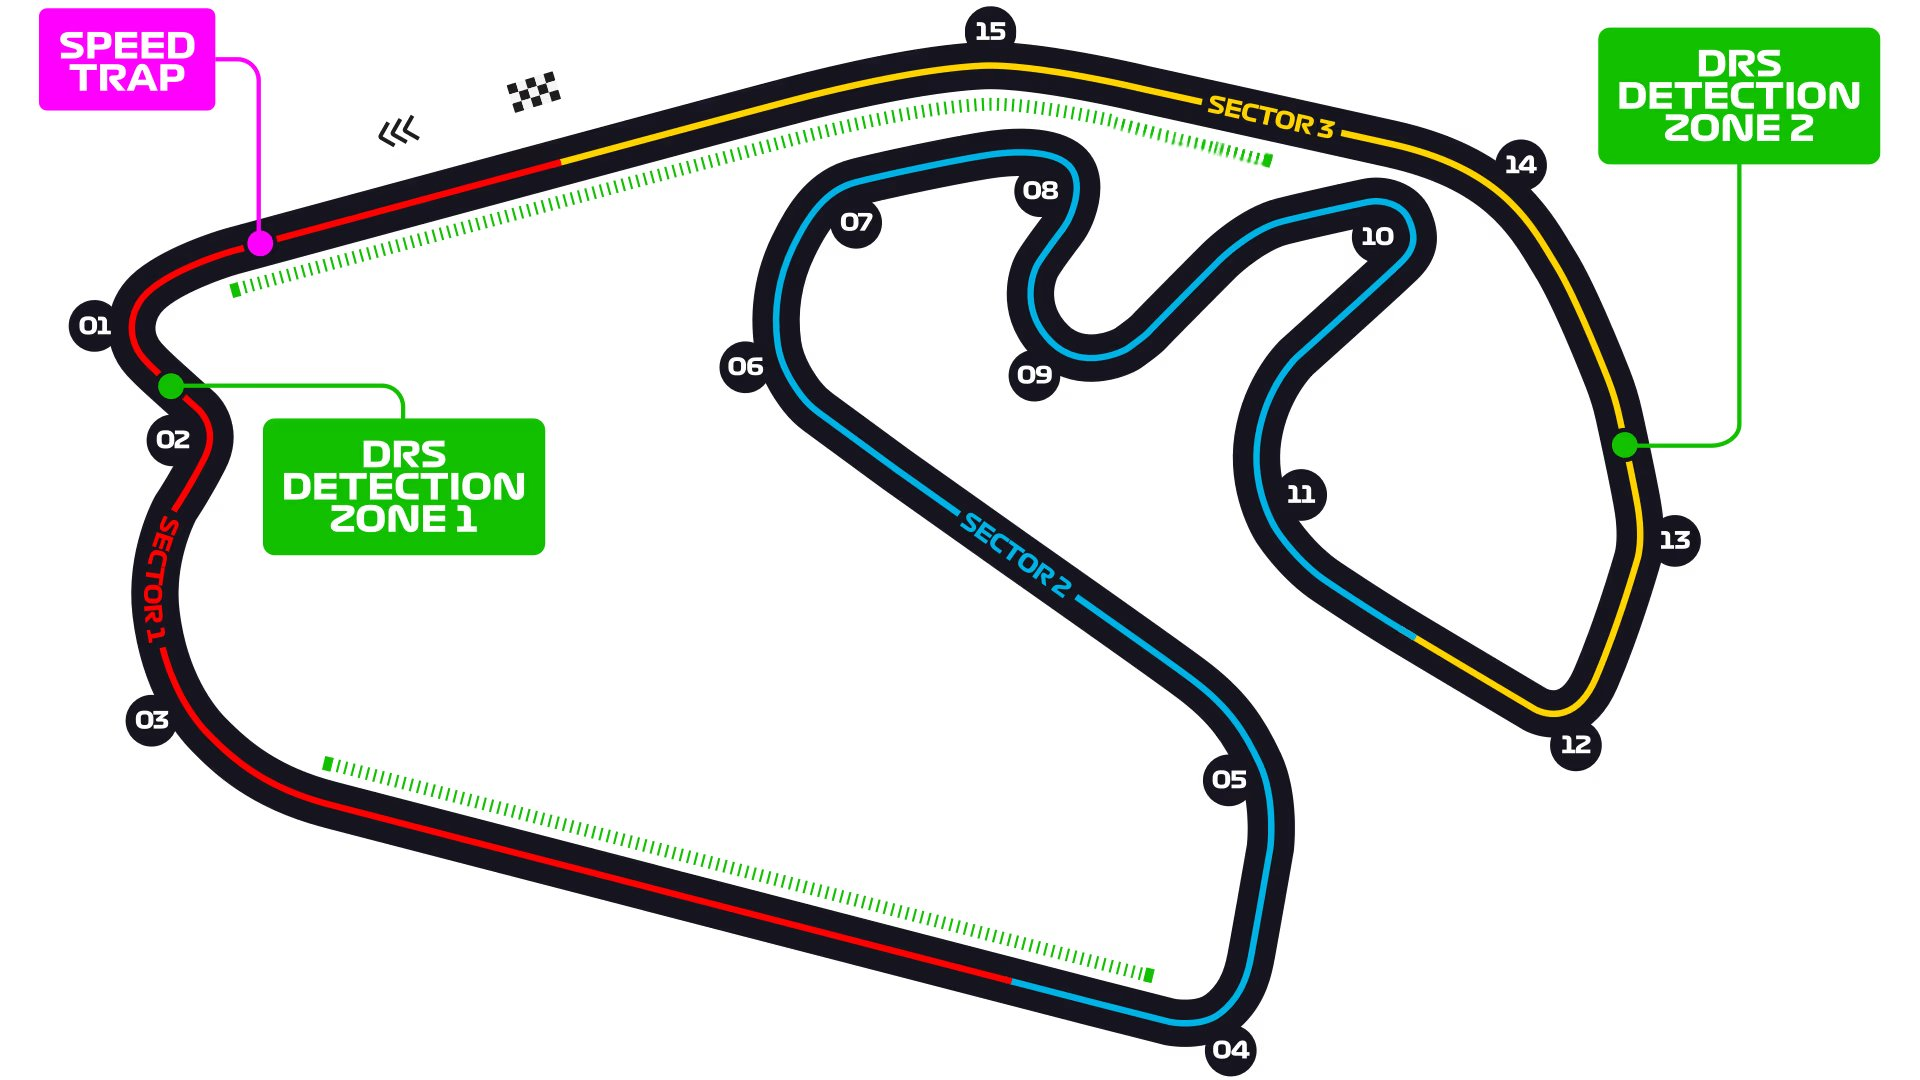
\includegraphics[width=0.75\linewidth]{images/21.Brazil_Circuit.jpg}
\end{figure}

\begin{itemize}
    \item \textbf{Lap Record} : 1:07.281 (2018, Lewis Hamilton – Mercedes).
    
    \item \textbf{Number of Corners \& Key Features} : 15 turns (5 right, 10 left). \\
    Counter-clockwise layout, famous for “Senna S” (Turns 1–2) and long uphill straight. \\
    High altitude + bumpy surface increase mechanical stress.
    
    \item \textbf{Braking Zones \& Traction} : Turn 1 (Senna S) heavy braking, prime overtaking zone. \\
    Traction critical at Juncão (Turn 12) leading to full-throttle run to finish line.
    
    \item \textbf{DRS \& Overtaking} : Two DRS zones (main straight and between Turns 3–4). \\
    Turn 1 and Turn 4 are the main overtaking opportunities.
    
    \item \textbf{Tyre Degradation \& Strategy} : High degradation due to track abrasiveness and elevation. \\
    Two-stop strategy typical, though weather chaos often dictates.
    
    \item \textbf{Weather \& Environment} : São Paulo notorious for sudden rain showers. \\
    Thin air reduces engine power, unpredictable conditions play major role.
\end{itemize}

\textbf{Strategic Summary :} Interlagos combines altitude challenges, mixed-speed corners, and unpredictable weather. Start and tyre strategy are critical; race often decided by timing of pitstops and Safety Cars.

\subsection{Race Analysis}

\textbf{Date:} Sprint : 2 November 2024 - 11:00 local time\\
Race : 3 November 2024 — 12:00 local time 

\begin{itemize}
    \item \textbf{Sprint Qualifying:} \textbf{Pole Position:} Oscar Piastri (McLaren) - 1:08.899.\\
    Grid : Norris 2nd, Leclerc 3rd, Verstappen 4th.
    
    \item \textbf{Sprint Summary} : \textbf{Winner:} Lando Norris (McLaren). \\
    \textbf{Podium:} 1. Norris - 2. Piastri - 3. Leclerc. \\
    Verstappen penalised 5s → dropped to P4.
    
    \item \textbf{Qualifying Summary} : Chaotic wet session with 5 red flags. \\
    \textbf{Pole Posision:} Lando Norris (McLaren) – 1:23.405. \\
    Grid : Russell 2nd, Tsunoda 3rd, Ocon 4th. \\
    Lawson P5, Leclerc P6. Verstappen only P12, dropped to P17 with engine penalty. Albon crashed in Q3 → DNS.
    
    \item \textbf{Race Summary} : \textbf{Winner:} Max Verstappen (Red Bull) — stunning recovery from P17. \\
    \textbf{Podium:} 1. Verstappen - 2. Ocon - 3. Gasly. \\
    Race started under rain, multiple Safety Cars and a red flag. \\
    Russell led first 28 laps, then Ocon/Gasly stayed out in worsening rain and temporarily led. \\
    After restart, Verstappen passed Ocon at Turn 1 (lap 43) and pulled away, also taking fastest lap. \\
    Norris struggled, finished only P6. Double Alpine podium, first since Spain 1997 with two French drivers.
    
    \item \textbf{Notable Incidents} : \\
    - Lap 1: Stroll spun off during formation, DNS. \\
    - Lap 27: Heavy rain → mass pitstops, Ocon and Gasly stayed out. \\
    - Lap 30: Colapinto big crash → red flag. \\
    - Lap 38: Sainz crashed → Safety Car. \\
    - Lap 43: Verstappen overtakes Ocon for the lead. \\
    - Piastri + Bearman penalised 10s for contacts. Hülkenberg disqualified after receiving external help.
    
    \item \textbf{Strategies} : \\
    - Verstappen: intermediate → wet → slicks, perfectly timed, + fastest lap. \\
    - Ocon/Gasly: bold gamble staying out before red flag, secured podiums. \\
    - Mercedes: Russell led early but faded, finished P4; Hamilton P10 after recovery. \\
    - McLaren: Norris lost momentum with off-track moment, P6. Piastri penalised, P8. \\
    - Ferrari: Leclerc P5 solid, Sainz retired in crash. \\
    - Racing Bulls: Tsunoda P7, Lawson P9. \\
    - Haas: Bearman penalised, P12; Hülkenberg DSQ.
    
    \item \textbf{Performance Trends} : \textbf{Red Bull} back on top with Verstappen’s comeback. \\
    \textbf{Alpine} revived with double podium, showing opportunistic strategy. \\
    \textbf{McLaren} lacked composure in chaos, Ferrari steady but unspectacular. \\
    \textbf{Mercedes} strong start but couldn’t sustain. \\
    \textbf{Williams} collapsed after Albon DNS and Colapinto crash. 
    
    \item \textbf{Championship Impact} : \textbf{Drivers:} Verstappen 393 pts, Norris 331, Leclerc 307. \\
    \textbf{Constructors:} McLaren 593, Ferrari 557, Red Bull 544, Mercedes 382. \\
    Verstappen can clinch title at next race in Las Vegas.
\end{itemize}

\textbf{Key Takeaway :} Verstappen produced one of his greatest wins, storming from P17 to victory in chaotic São Paulo conditions. Alpine shocked the paddock with a double podium, McLaren faltered, and Mercedes/Ferrari lacked decisive pace. Championship battle tightened in constructors, but Verstappen now holds the drivers’ crown within reach.

\subsection{Link \& Takeaway}

\begin{itemize}
    \item Interlagos delivered another chaotic thriller: rain, Safety Cars, red flag, and late drama. 
    \item Verstappen showcased racecraft and adaptability, turning a P17 start into a commanding win. 
    \item Alpine’s opportunism rewarded with a historic French double podium, a rare highlight in their season. 
    \item McLaren slipped under pressure, Ferrari stayed consistent, Mercedes missed podium chance. 
    \item The result leaves Verstappen with one hand on the drivers’ trophy, while constructors’ title fight remains wide open. 
\end{itemize}
